%!TEX root = ../thesis.tex
%Adding the above line, with the name of your base .tex file (in this case "thesis.tex") will allow you to compile the whole thesis even when working inside one of the chapter tex files

\chapter{Discrete Absorption Feature}\label{app:2}

During this study we analyzed \textit{HST} STIS spectra of Arcturus from the online StarCAT catalog \citep{ayres_2010}. The \ion{Mg}{ii} h and k lines from data obtained in 2001 show a wind velocity $ \thicksim 30-40 \ \rm{km \ s^{-1}}$, which is similar to that adopted in the Drake models for this star \cite{drake_1985}. A narrow discrete absorption feature was found at $-49 \ \rm{km \ s^{-1}}$ in the broad blue-shifted wind absorption component of both lines as shown in Figure \ref{fig:app2}. For this discrete feature we find a most probable turbulent velocity of $ 3.4 \ \rm{km \ s^{-1}}$ and a \ion{Mg}{ii} column density\footnote{Assuming all Mg to be Mg II} of $1.4\times10^{12}$\, cm$^{-2}$. A \ion{Mg}{ii} column density of $10^{15}$\, cm$^{-2}$ is required to produce the blueward absorption components in the \textit{h} and \textit{k} lines \citep{mcclintock_1978}. Therefore, this discrete absorption feature accounts for only $\thicksim 0.1 \%$ of the total wind column density and is probably a result of a discrete ejection event.

\begin{figure}[hb!]
\centering 
\mbox{
          \includegraphics[trim=30pt 10pt 10pt 0pt,clip,width=7.2cm, height=13.0cm]{/home/eamon/thesis/thesis_template/appendix/ogorman_e_fig6.eps} 
          \includegraphics[trim=30pt 10pt 10pt 0pt,clip,width=7.2cm, height=13.0cm]{/home/eamon/thesis/thesis_template/appendix/ogorman_e_fig7.eps}
          }
\caption[]{Analysis on the absorption feature found in the \ion{Mg}{ii} \textit{h} and \textit{k} lines. A function composed of a linear combination of a Gaussian and a quadratic fitted the discrete absorption feature the best. The red data in the upper row shows the data that is used in this analysis.}
\label{fig:app2}
\end{figure}